\section{Organisations existantes}
Il sera présenté ici un rassemblement d'initiatives similaires à ce travail. Ces initiatives sont toutes non-gouvernementales et propose d'enseigner la programmation de différente manières. C'est sur ce dernier point que l'accent sera mis dans la suite de ce tour des organisations.
\subsection{Code.org}
\begin{figure}[!h]
  \begin{center}
    
\includegraphics[scale=0.5]{content/5-related_work/images/code}
    \caption{Logo de code.org}
    \label{fig:code.org}
  \end{center}
\end{figure}
Code.org\footnote{\url{http://code.org/about}} est une organisation sans but lucratif des USA qui à pour objectifs :
\begin{itemize}
  \item apporter l'informatique dans toutes les classes de secondaire aux USA ;
  \item démontrer le succès de l'utilisation de cours en ligne dans l'enseignement public ;
  \item ajouter l'informatique dans les bases des programmes de sciences et de mathématique des 50 états ;
  \item employé la connaissance technique collective pour améliorer l'apprentissage de l'informatique dans le monde ;
  \item augmenter la représentation féminine et des personnes de couleurs dans informatique.
\end{itemize}

Pour ce faire, ils fournissent une plate forme\footnote{\url{http://code.org/educate/20hr}} web qui permet aux professeurs de suivre leurs élèves grâce à un système de classe.

Toutes les ressources sont gratuites et librement utilisables\footnote{\url{http://code.org/faq}}. Leur programme d'apprentissage se base sur Blockly (voir \ref{blockly}).
Les ressources sont conçues pour que les professeurs comme les étudiants puissent commencer le cours sans connaître l'informatique (une assistance est proposée au professeur gratuitement si nécessaire).

Le site propose aux professeurs de se faire récompenser s'ils arrivent à finir les 27 missions proposées à minimum 15 étudiants. Dans ce cas, ils gagnent $750\$$, s'ils ont au moins 7 filles dans le groupe ils peuvent prétendre à $250\$$ supplémentaire.

\subsubsection{Déroulement des leçons}
Il propose des sessions de une heure de travail/jeu/apprentissage. Chaque unité d'une heure est découpée en petite mission (ex:5-20) les missions sont très courte et apporte un concept de programmation. Avant l'introduction de chaque concept, une petite vidéo est faite pour expliquer le concept introduit et des exemples de ce que la programmation permet de réaliser avec ce dernier.

Ils proposent de faire travailler les étudiants par pair\footnote{pair programming \url{http://en.wikipedia.org/wiki/Pair\_programming}}. Ceci permet d'avoir moins de questions pour le professeur et de mieux s'approprier la matière. Le travail par pair permet également de casser l'image du "geek" en montrant que la programmation est une science sociale et collaborative. Sans oublier qu'avec deux enfants par station, moins d'ordinateurs seront nécessaires.

Le site explique également que pour faire participer tout les élèves, il faut avoir confiance en leur compétence : permettre aux premiers groupes d'aider les derniers.

Quand un étudiant a une question, ils recommandent de proposer aux étudiants de d'abord demander à 3 de leurs camarades avant de poser la question au professeur. Le professeur ne devant pas être compétent, il doit juste pouvoir réfléchir avec les élèves de quel est le problème, cela permet aussi d'évité les questions de distraction ou de manque de compréhension.

Pour chaque petite mission, il y a un test automatisé qui dit si la mission est réussie ou non. Si la mission est réussie, le programme passe à la mission suivante. Il y a également un compteur de blocs dans les premières missions. Ce compteur permet de voir combien de blocs sont nécessaires pour réaliser la mission de manière optimale.

\subsection{CoderDojo}
\begin{figure}[!h]
  \begin{center}
    
\includegraphics[scale=0.5]{content/5-related_work/images/dojo}
    \caption{Logo de CoderDojo}
    \label{fig:coder dojo}
  \end{center}
\end{figure}
CoderDojo\footnote{\url{http://coderdojo.com/about}} est un réseau open source de clubs de programmation dans le sens le plus large du terme. Tous les dojos sont donc autonomes. Dans ceux-ci, des enfants de 5 à 17 ans apprennent la programmation (site web, application, jeux...). La seul règle est "Above All : Be Cool" qui peut être mis en pratique simplement en créant des espaces d'échanges de savoir amical et sociable.

CoderDojo a été crée par James Whelton un irlandais de 18 ans et Bill Liao un entrepreneur australien à Cork. James a eu des demandes de jeunes enfants pour avoir des cours de programmation après qu'il eut hacké l'iPod nano. Beaucoup de gens de Dublin vinrent à ses cours et donc un nouveau Dojo a été créé à Dublin et puis cela s'est étendu à tout le globe.

\subsection{Code Club}
\begin{figure}[!h]
  \begin{center}
    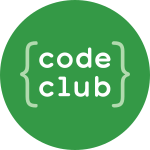
\includegraphics[scale=0.3]{content/5-related_work/images/club}
    \caption{Logo de Code Club}
    \label{fig:code club}
  \end{center}
\end{figure}
Code Club\footnote{\url{https://www.codeclub.org.uk/about}} est un réseau de clubs national mené par des bénévoles en dehors des heures de cours. Ces activités s'adressent à des enfants de 9 à 11 ans.

Ils créent donc le matériel pour permettre à des bénévoles de donner des cours parascolaires d'environ une heure semaine. Il propose dans l'ordre d'utiliser scratch, HTML/css et puis Python. Ils aimeraient que les 21000 écoles primaires anglaises aient leur club.

Leur philosophie est de d'abord l'amusement, la créativité et l'exploration avant l'apprentissage des concepts de programmation.
